\documentclass{article}
\usepackage[paperwidth=6in, paperheight=9in, margin=0.75in]{geometry}
\usepackage{fontspec}
\usepackage{xcolor}
\usepackage{graphicx}
\usepackage{tikz}

% Set up fonts
\setmainfont[Script=Devanagari] {Tiro Devanagari Marathi}
\newfontfamily\devanagarifont[Scale=MatchUppercase]{Tiro Devanagari Marathi}
%\setmainfont[Script=Devanagari]{Nirmala Text}
%\newfontfamily\devanagarifont[Scale=MatchUppercase]{Nirmala Text}
% \setmainfont[Script=Devanagari]{Noto Serif Devanagari}
% \newfontfamily\devanagarifont[Scale=MatchUppercase]{Noto Serif Devanagari}

\newfontfamily\devtransl[Mapping=DevRom]{Segoe UI}
\graphicspath{{images/}}

% Define colors
\definecolor{titleorange}{RGB}{255,140,0}
\definecolor{subtitleblue}{RGB}{0,51,102}
\definecolor{authorgreen}{RGB}{0,102,51}

\pagestyle{empty}

\begin{document}

% FRONT COVER PAGE
\thispagestyle{empty}
\null\vfill

\begin{center}
% Title - big orange font, 60% page width
{\fontsize{58}{78}\selectfont\color{titleorange}\textbf{एआय-रूपे}}

\vspace{1em}

% Subtitle - quarter size, dark blue
{\fontsize{12}{14}\selectfont\color{subtitleblue}('कृत्रिम बुद्धिमत्ते'ची विविध क्षेत्रातील रूपे)}

\vspace{5em}

% Author - dark green
{\fontsize{16}{20}\selectfont\color{authorgreen}\textbf{डॉ. योगेश हरिभाऊ कुलकर्णी}}
\end{center}

\vfill\null
\clearpage

% BACK COVER PAGE
\thispagestyle{empty}
\vspace*{0.5in}

% Book description
\noindent\textbf{पुस्तकाविषयी:} या पुस्तकात कृत्रिम बुद्धिमत्तेच्या विविध क्षेत्रातील रूपांचा सविस्तर अभ्यास करण्यात आला आहे. तंत्रज्ञान, वैद्यकीय शास्त्र, शिक्षण, व्यवसाय आणि दैनंदिन जीवनातील एआय च्या उपयोगांचे विश्लेषण करून, भविष्यातील शक्यता आणि आव्हानांवर प्रकाश टाकला आहे.  या पुस्तकाचे उद्दिष्ट कृत्रिम बुद्धिमत्तेची जटिल संकल्पना सामान्य वाचकांपर्यंत सुलभ मराठी भाषेत पोहोचवणे आहे. तंत्रज्ञान क्षेत्रातील नवीन विकास आणि त्यांचा समाजावरील परिणाम यांचे तर्कसंगत विश्लेषण या पुस्तकाची खासियत आहे.

\vspace{1.5em}

% Target audience
\noindent\textbf{वाचकांविषयी:} तंत्रज्ञानात रस असणाऱ्या सर्वांसाठी हे पुस्तक योग्य आहे.

\vspace{1.5em}

% Author bio
\noindent\textbf{लेखकाविषयी: डॉ. योगेश हरिभाऊ कुलकर्णी} हे तंत्रज्ञान क्षेत्रातील अनुभवी अभ्यासक आहेत. त्यांना कृत्रिम बुद्धिमत्ता, मशीन लर्निंग आणि डेटा सायन्स या क्षेत्रात अनेक वर्षांचा अनुभव आहे. शैक्षणिक क्षेत्रात तसेच उद्योगात काम करून त्यांनी या विषयावर व्यापक अभ्यास केला आहे. त्यांचे पूर्वीचे लेखन कार्य आणि संशोधन हे मराठी भाषेत तंत्रज्ञान विषयक साहित्याला वाव देण्याच्या दिशेने योगदान आहे.

\vfill

% Author photo and contact info at bottom
\begin{tabular}{@{}p{0.3\textwidth}@{}p{0.2\textwidth}@{}p{0.3\textwidth}@{}}
\centering
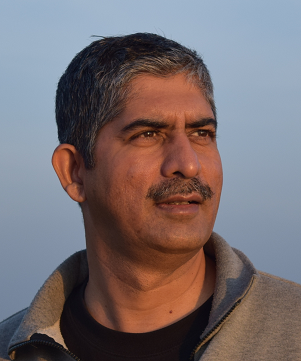
\includegraphics[width=\linewidth,keepaspectratio]{myphoto} 

yogeshkulkarni@yahoo.com
&
% blank column &
& 
\centering
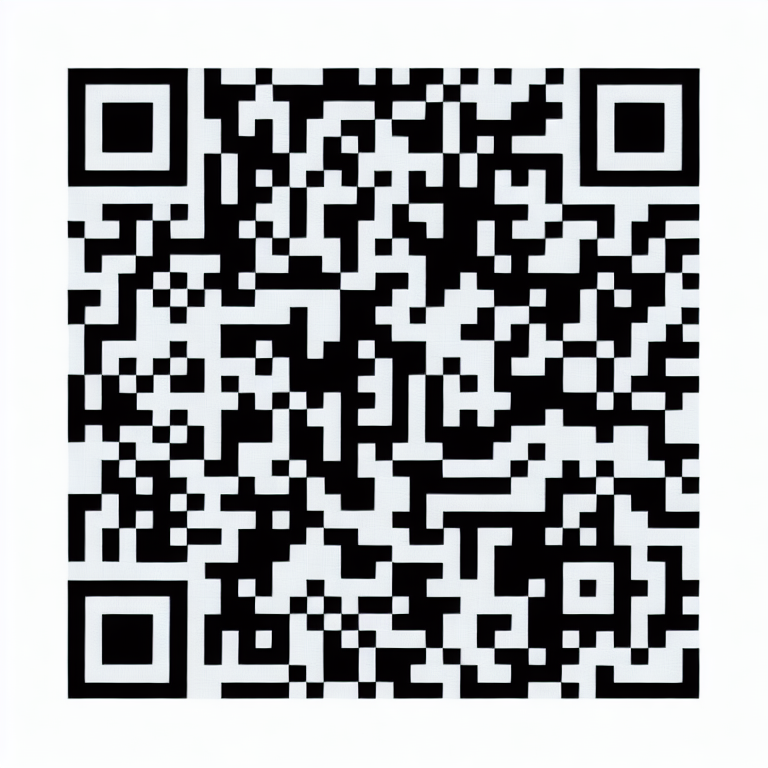
\includegraphics[width=\linewidth,keepaspectratio]{mylinkedinqr}

+91 9890251406
\end{tabular}


% Publisher info at bottom
\begin{center}
\textbf{[प्रकाशकाचे नाव]}\\
\texttt{www.[publisher-website].com}\\
ISBN: [ISBN नंबर]
\end{center}

\begin{center}
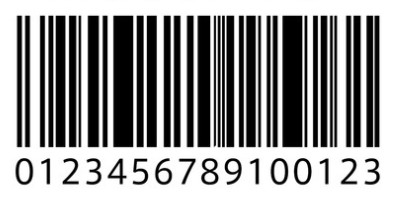
\includegraphics[width=3cm]{isbn_barcode}
\end{center}

\end{document}